\documentclass{article}
\usepackage[utf8]{inputenc}
\usepackage{geometry}
 \geometry{
 a4paper,
 total={170mm,257mm},
 left=20mm,
 top=20mm,
 }
\usepackage{polski}
\usepackage{natbib}
\usepackage[capbesideposition=right]{floatrow}
\usepackage{graphicx}
\usepackage{pbox}
\usepackage{float}
\usepackage[dvipsnames]{xcolor}
\usepackage{caption}
\usepackage{wrapfig}
\usepackage{graphicx}
\usepackage{tikz}
    \usetikzlibrary{
        arrows,
        shadows,
        shapes,
        automata,
        positioning,
        arrows.meta
    }
\usepackage{pgfplots}
\usepackage{tabularx}
\usepackage{booktabs}
\usepackage{amsfonts}
\pgfplotsset{compat=1.17}

\begin{document}
\centering 
\Huge Activity diagram of a single turn
\vspace{1cm}
\normalsize
    
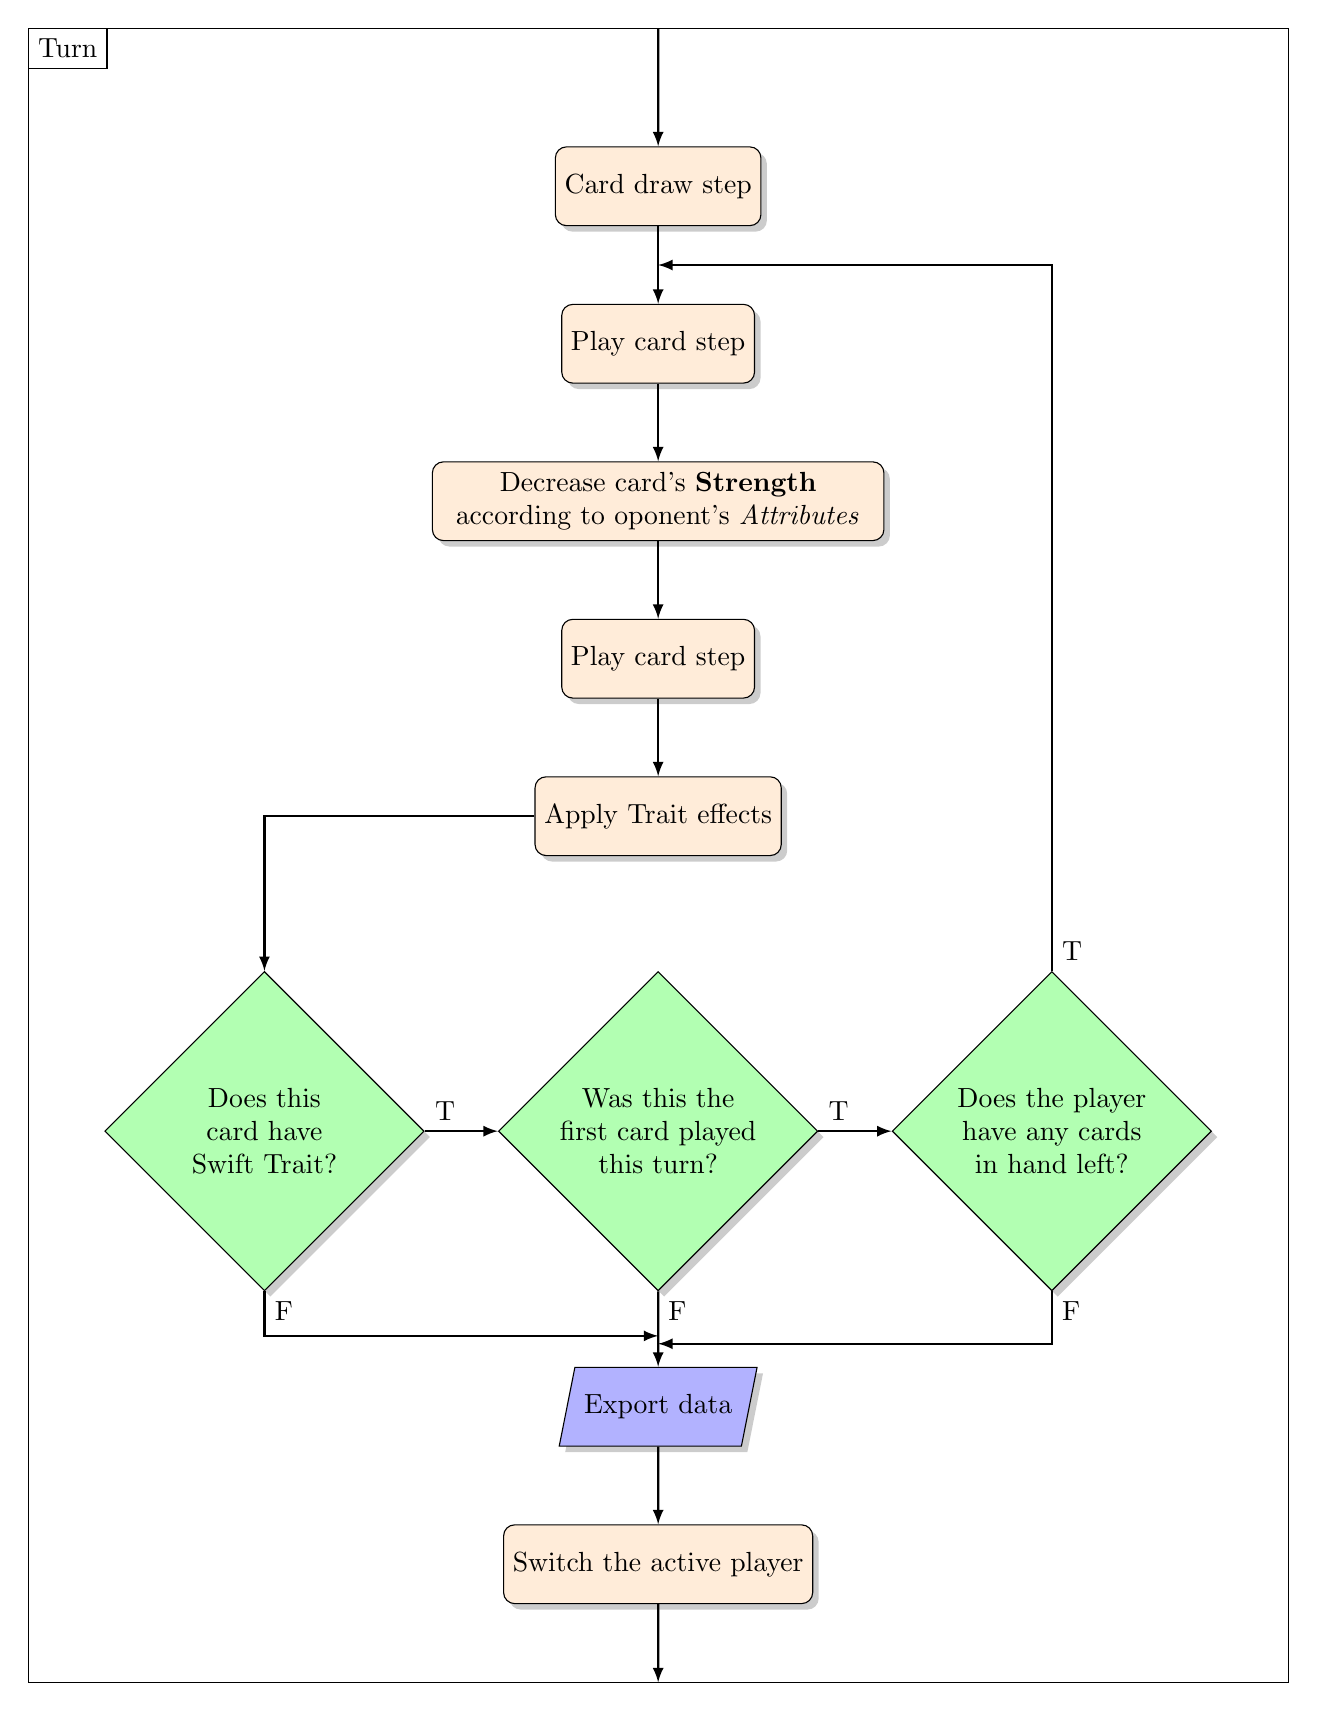
\begin{tikzpicture}
[baseshape/.style={minimum width=1.5cm, minimum height=1cm,text centered, font=\normalsize,draw=black, drop shadow=black!40},
startstop/.style={baseshape, ellipse, fill=red!30},
io/.style={baseshape, trapezium, trapezium stretches=true, 
trapezium left angle=70, trapezium right angle=110, fill=blue!30},
process/.style={baseshape, rectangle, rounded corners, fill=orange!15},
decision/.style={baseshape, diamond, minimum width=1cm, fill=green!30, text width=2.5cm},
block/.style={baseshape, rectangle, minimum width=1cm, fill=white},
arrow/.style={thick, -latex},
node distance=2cm,]
\node (step0) [process, xshift = 3cm, yshift = -1cm] {Card draw step};
\node (step1) [process, below of = step0] {Play card step};
\node (step2) [process, below of = step1, text width = 5.5cm] {Decrease card's \textbf{Strength} \\ according to  oponent's \textit{Attributes}};
\node (step3) [process, below of = step2] {Play card step};
\node (step4) [process, below of = step3] {Apply Trait effects};
\node (step5) [decision, below of = step4, yshift = -2cm, xshift = -5cm ] {Does this card have Swift Trait?};
\node (step5a) [decision, right of = step5, xshift = 3cm] {Was this the first card played this turn?};
\node (step5b) [decision, right of = step5a, xshift = 3cm] {Does the player have any cards in hand left?};
\node (step6) [io, below of= step5a, yshift = -1.5cm] {Export data};
\node (step7) [process, below of = step6] {Switch the active player};
\draw (-5,1) -- node[at start, anchor=north west]{Turn}(-4,1) -- (-4, 0.5) -- (-5, 0.5) -- (-5, 1) -- (11, 1) -- (11, -20) -- (-5,-20) -- (-5, 1);
\draw[arrow] (3, 1) -- (step0);
\draw[arrow] (step0) -- (step1);
\draw[arrow] (step1) -- (step2);
\draw[arrow] (step2) -- (step3);
\draw[arrow] (step3) -- (step4);
\draw[arrow] (step4) -| (step5);
\draw[arrow] (step5) -- node[at start, anchor=south west]{T}(step5a);
\draw[arrow] (step5a) -- node[at start, anchor=south west]{T}(step5b);
\draw[arrow] (step5b) |- node[at start, anchor=south west]{T}(3, -2);
\draw[arrow] (step5a) -- node[at start, anchor=north west]{F}(step6);
\draw[arrow] (step6) -- (step7);
\draw[arrow] (step7) -- (3, -20);

\draw[arrow] (step5) |- node[at start, anchor=north west]{F}(3, -15.6);
\draw[arrow] (step5b) |- node[at start, anchor=north west]{F}(3, -15.7);

\end{tikzpicture}
\end{document}